%Template file for MATH96012 project 1 discussion and figures
\documentclass{article}
\usepackage[utf8]{inputenc}
\title{MATH96012 Project 1}

\author{\emph{Alexander John Pinches CID:01201653}}

\usepackage{graphicx}
\usepackage{amsmath}
\begin{document}

\maketitle

%---------------- Question 2 -------------------

\section*{Part 2}
\subsection{2.1}
We see in figure \ref{fig1} variability in $\alpha$ seems to increase as we increase $A$. This would make sense as increasing $A$ increases the effect of the random component of the directions of the particles. $\alpha$ initially varies lots before becoming more stationary this seems to happen after the first 50 or so time steps. We can remove the initial transient and use a high Nt to reduce the effect of this. For $N=32$ there seems to be less variation. We would expect this as more particles interacting with each other should force them into alignment faster.There also seems to be a point where the variability of the series changes rapidly with $A=0.2$ being almost constant after the initial transient. The variability in the $N=16$ series seems to increase more as we increase $A$ this is most noticible when $A=0.6$. If we use the variance and mean after the initial 50 time points in figure \ref{fig2} the dotted lines represent the mean plus and minus two times the standard deviation. We see that mean $\alpha$ seems similar for both $N=16,32$ but the width of the dotted bars around the mean are smaller suggesting that the variability of $\alpha$ is smaller. We also see that the width increases from 0.2 to about 0.6 then reduces again as $A$ reaches 0.8 suggesting there's a point around 0.6 where the variability of $\alpha$ is greatest. We can also see this in figure \ref{fig3} that the variance has a maximum at $A=0.6$ and that the variance of $N=16$ is higher than that of $N=32$. with both increasing rapidly from $A=0.4$ to $A=0.6$.

\subsection{2.2}
When trying to find $A^{*}$ using the minimise function from scipy on the negative variance of $A$ would find solutions outside the bounds or for methods we can bound they wouldn't converge or explore the space. Instead I opted to just perform a grid search of the parameter space as for $N=32$ and $Nt=1000$ this is still rather fast even when searching 1201 points. Allowing us to get of an estimate of $A^{*}$ down to the 0.005. However, due to the stochastic nature of the system in general the result is similar between runs it can differ.In figure \ref{fig4} we plot $\mathrm{Var}[\alpha]$ against $A$ and we mark $A^{*}$ with a blue dot. We see that the variance of $\alpha$ increases slowly then rapidly up from 0.6 and down again after which is what we expect from the plot in figure \ref{fig4}. We could maybe apply some filter to remove the noise or fit a curve and take the max of that but whether this is actually anymore accurate I am unsure.
\\

To see the dependence of $\alpha$ on $1 - \frac{A}{A^{*}}$ we plot them against each other figure \ref{fig5}. Showing the mean $\alpha$ as a red line and the plus and minus two times the standard deviation as blue dashed lines. We see as $1 - \frac{A}{A^{*}}$ increases the variation decreases and the mean increases which is as we would expect as alpha varies most when $A$ is close to $A^{*}$.  We see close to 0 ie when $A$ is close to $A^{*}$ the variation in alpha increases rapidly as we would expect. To see this better in figure \ref{fig6} we plot $\mathrm{Var}[\alpha]$ against  $1 - \frac{A}{A^{*}}$ and see the variance increases asymptotically as $1 - \frac{A}{A^{*}} \xrightarrow{}{} 0$ and rapidly approaches 0 as it moves to the right.

\subsection*{Figures}
\begin{figure}[h!]
\centering

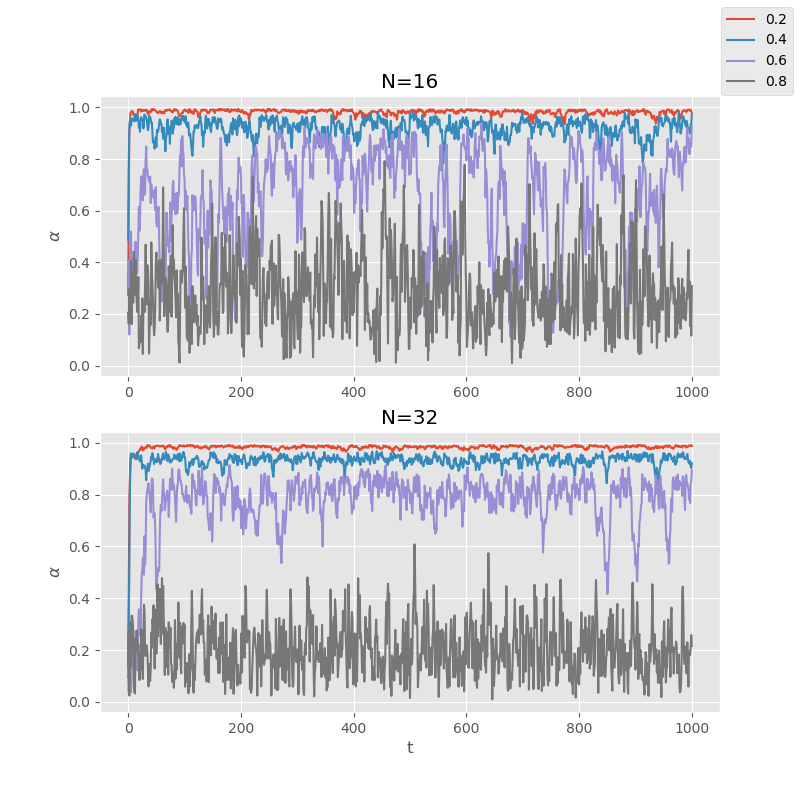
\includegraphics[width=0.6\textwidth]{alphaTime.png}
\caption{$\alpha$ over time for $N=16,32$}
\label{fig1}
\end{figure}

\begin{figure}[h!]
\centering

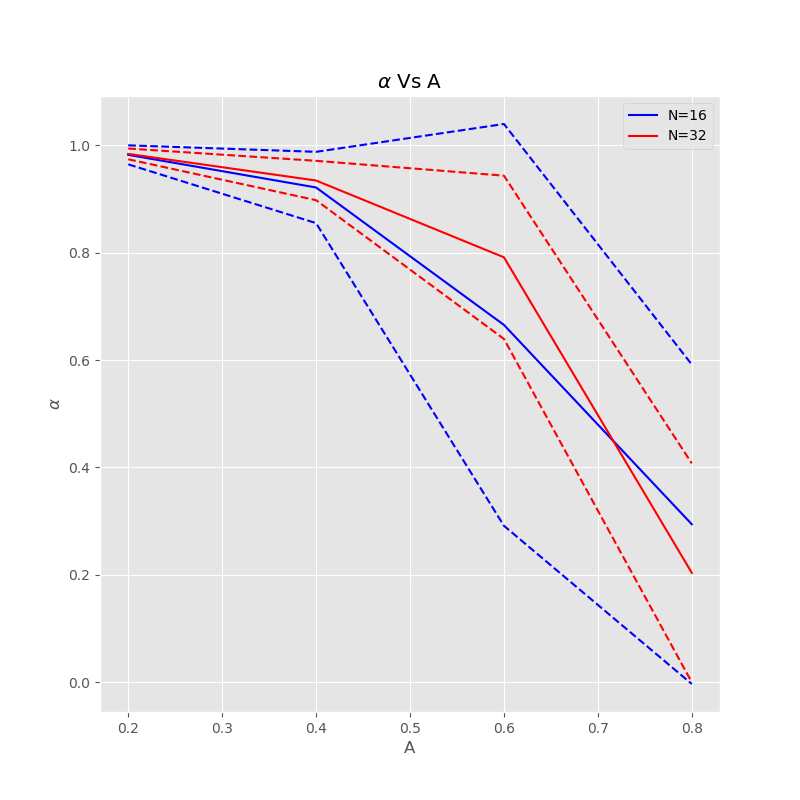
\includegraphics[width=0.6\textwidth]{alphaMean.png}
\caption{Mean $\alpha$ (red) for $N=16,32$ with first 50 steps omitted and $\pm2\sigma[\alpha]$ dotted lines over $A$}
\label{fig2}
\end{figure}

\begin{figure}[h!]
\centering

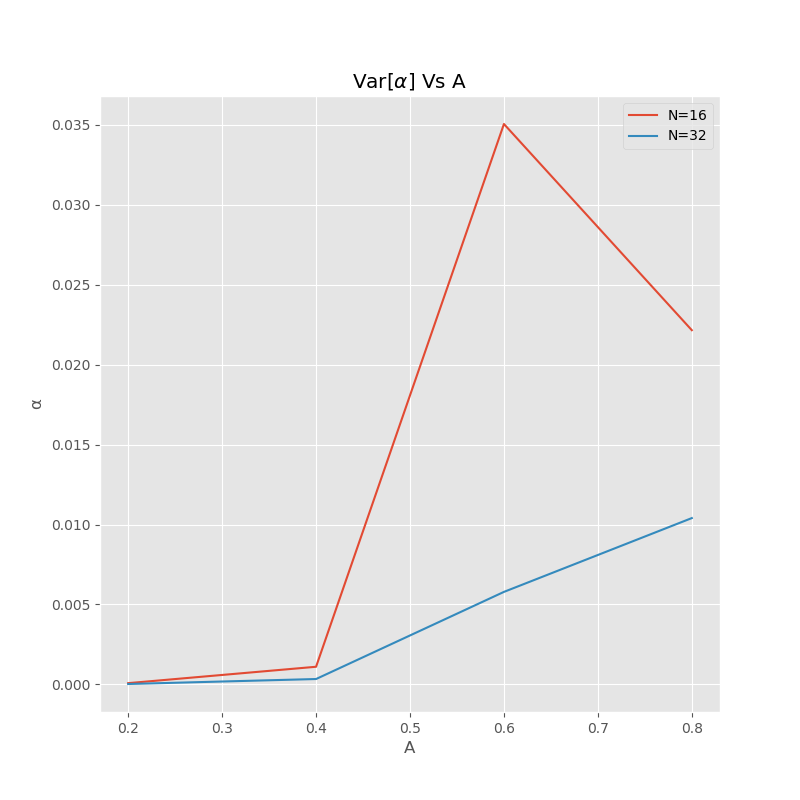
\includegraphics[width=0.6\textwidth]{alphaVar.png}
\caption{Variance of $\alpha$ against $A$ for $N=16,32$}
\label{fig3}
\end{figure}

\begin{figure}[h!]
\centering

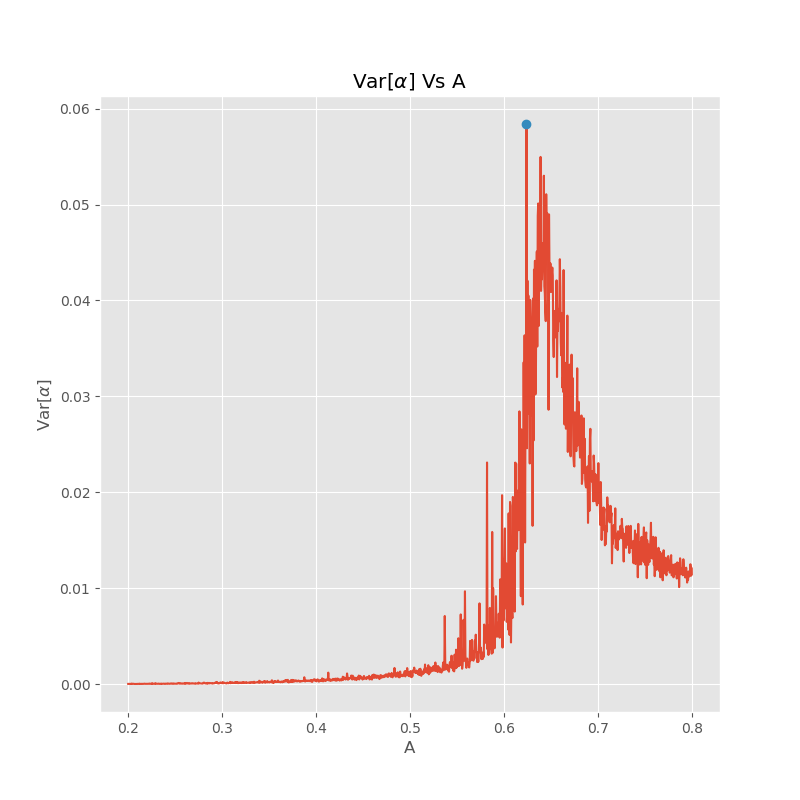
\includegraphics[width=0.6\textwidth]{rate.png}
\caption{$\mathrm{Var}[\alpha]$ against $A$ with $A^{*}$ represented by a blue dot}
\label{fig4}
\end{figure}

\begin{figure}[h!]
\centering

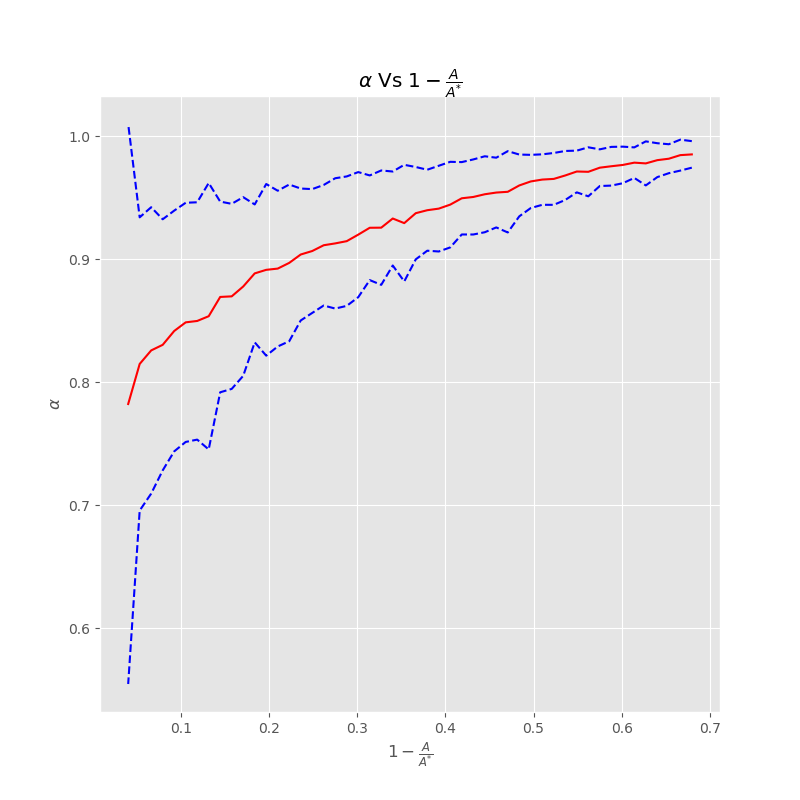
\includegraphics[width=0.6\textwidth]{alphaDependence.png}
\caption{Mean $\alpha$ with against $1 - \frac{A}{A^{*}}$}
\label{fig5}
\end{figure}

\begin{figure}[h!]
\centering

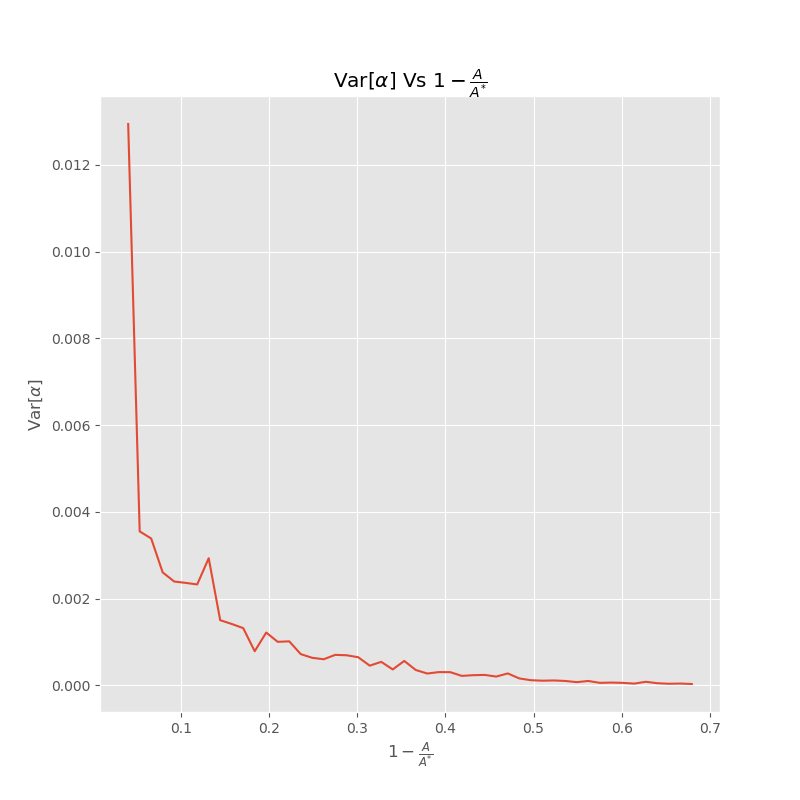
\includegraphics[width=0.6\textwidth]{alphaDependenceVar.png}
\caption{$\mathrm{Var}[\alpha]$ with $\pm2\sigma[\alpha]$ dotted lines against $1 - \frac{A}{A^{*}}$}
\label{fig6}
\end{figure}



%---------------- End Question 2 -------------------





%---------------- End document -------------------


\end{document}
